% !TEX program = xelatex
\documentclass[12pt,a4paper]{article}

% ---- Layout, spacing and line numbers ----
\usepackage[margin=2.5cm]{geometry}
\usepackage{setspace}
\usepackage[mathlines]{lineno}
\doublespacing
\linenumbers

% ---- Font: TeX Gyre Termes (bundled) ----
\usepackage{fontspec}
\setmainfont{TeX Gyre Termes}
\newfontfamily\headfont{TeX Gyre Heros}   % sans-serif for title, headings and captions

% ---- Packages ----
\usepackage{amsmath,amssymb}
\usepackage{graphicx}
\usepackage{booktabs}
\usepackage{titlesec}
\usepackage[font=small,labelfont=bf,labelsep=period,justification=raggedright,singlelinecheck=false]{caption}
\usepackage[numbers,sort&compress]{natbib}
\usepackage{xcolor}
\usepackage{hyperref}

\definecolor{linkblue}{HTML}{1F3A7A}
\hypersetup{colorlinks=true,linkcolor=linkblue,citecolor=linkblue,urlcolor=linkblue,pdftitle={Full Title of the Manuscript}}
\titleformat{\section}{\headfont\bfseries\large}{\thesection}{0.75em}{}
\titleformat{\subsection}{\headfont\bfseries\normalsize}{\thesubsection}{0.75em}{}
\titlespacing*{\section}{0pt}{2ex plus 0.5ex}{1ex}
\titlespacing*{\subsection}{0pt}{1.5ex plus 0.5ex}{0.5ex}
\DeclareCaptionFont{heros}{\headfont}
\captionsetup{labelfont={heros,bf}}
\renewcommand{\linenumberfont}{\normalfont\footnotesize}
\newcommand{\orcid}[1]{\href{https://orcid.org/#1}{ORCID: #1}}

% ---- Title block ----
\title{{\headfont\bfseries\Large Full Title of the Manuscript: A Concise and Informative Subtitle}}
\author{%
  First A. Author$^{1,*}$ (\orcid{0000-0000-0000-0000}) \\
  Second B. Author$^{2}$ (\orcid{0000-0000-0000-0000}) \\
  Third C. Author$^{1,2}$ (\orcid{0000-0000-0000-0000}) \\[6pt]
  \small $^{1}$Department, Institution, City, Country \\
  $^{2}$Department, Institution, City, Country \\[3pt]
  $^{*}$Corresponding author: First A. Author, Postal address \\
  \href{mailto:email@example.org}{email@example.org}, tel.\ +00 000 000 000}
\date{}

\begin{document}
\singlespacing   % no group around \maketitle: lineno breaks if a page ends inside one
\maketitle

\begin{abstract}
\singlespacing
\noindent\textbf{Background:} State the problem and why it matters.
\textbf{Methods:} Summarise the design, sample and analysis.
\textbf{Results:} Report the main quantitative findings.
\textbf{Conclusions:} State the principal conclusion and its implications
(250 words maximum).

\medskip
\noindent\textbf{Keywords:} keyword one; keyword two; keyword three; keyword four
\end{abstract}

\newpage
\doublespacing
\section{Introduction}\label{sec:intro}
Review the relevant literature and identify the gap~\cite{author2020,colleague2019}.
State the research question, the hypothesis and the contribution of this work.
The remainder of the paper is organised as follows: Section~\ref{sec:methods}
describes the methods, Section~\ref{sec:results} presents the results, and
Section~\ref{sec:discussion} discusses their implications.

\section{Methods}\label{sec:methods}
\subsection{Study design and participants}
Describe the study design, setting, eligibility criteria and ethical approval
(include the approval number and consent procedure where applicable).

\subsection{Measurements}
Define the outcome variables and instruments. The response of unit $j$ in
group $i$ is modelled as
\begin{equation}\label{eq:model}
  y_{ij} = \mu + \tau_i + \varepsilon_{ij}, \qquad
  \varepsilon_{ij} \sim \mathcal{N}(0,\sigma^2),
\end{equation}
where $\mu$ is the grand mean and $\tau_i$ is the effect of group $i$.

\subsection{Statistical analysis}
Group differences are summarised by the standardised effect size
\begin{equation}\label{eq:effect}
  d = \frac{\bar{y}_1 - \bar{y}_2}{s_p}, \qquad
  s_p^2 = \frac{(n_1-1)s_1^2 + (n_2-1)s_2^2}{n_1+n_2-2},
\end{equation}
reported with 95\% confidence intervals. State the software, significance level
and handling of missing data. Equation~\eqref{eq:model} is extended in
Appendix~\ref{app:details}.

\section{Results}\label{sec:results}
\subsection{Descriptive statistics}
Table~\ref{tab:summary} summarises the sample. Replace the placeholder values
with your own results.

\begin{table}[htbp]
  \centering
  \caption{Summary statistics by group (placeholder values).}\label{tab:summary}
  \begin{tabular}{lccc}
    \toprule
    Group & $n$ & Mean $\pm$ SD & $p$ \\
    \midrule
    Control     & 00 & 0.0 $\pm$ 0.0 & --- \\
    Treatment A & 00 & 0.0 $\pm$ 0.0 & 0.000 \\
    Treatment B & 00 & 0.0 $\pm$ 0.0 & 0.000 \\
    \bottomrule
  \end{tabular}
\end{table}

\subsection{Time course and association}
Figure~\ref{fig:timecourse} shows the response over time, and
Figure~\ref{fig:scatter} shows its association with exposure.

\begin{figure}[htbp]
  \centering
  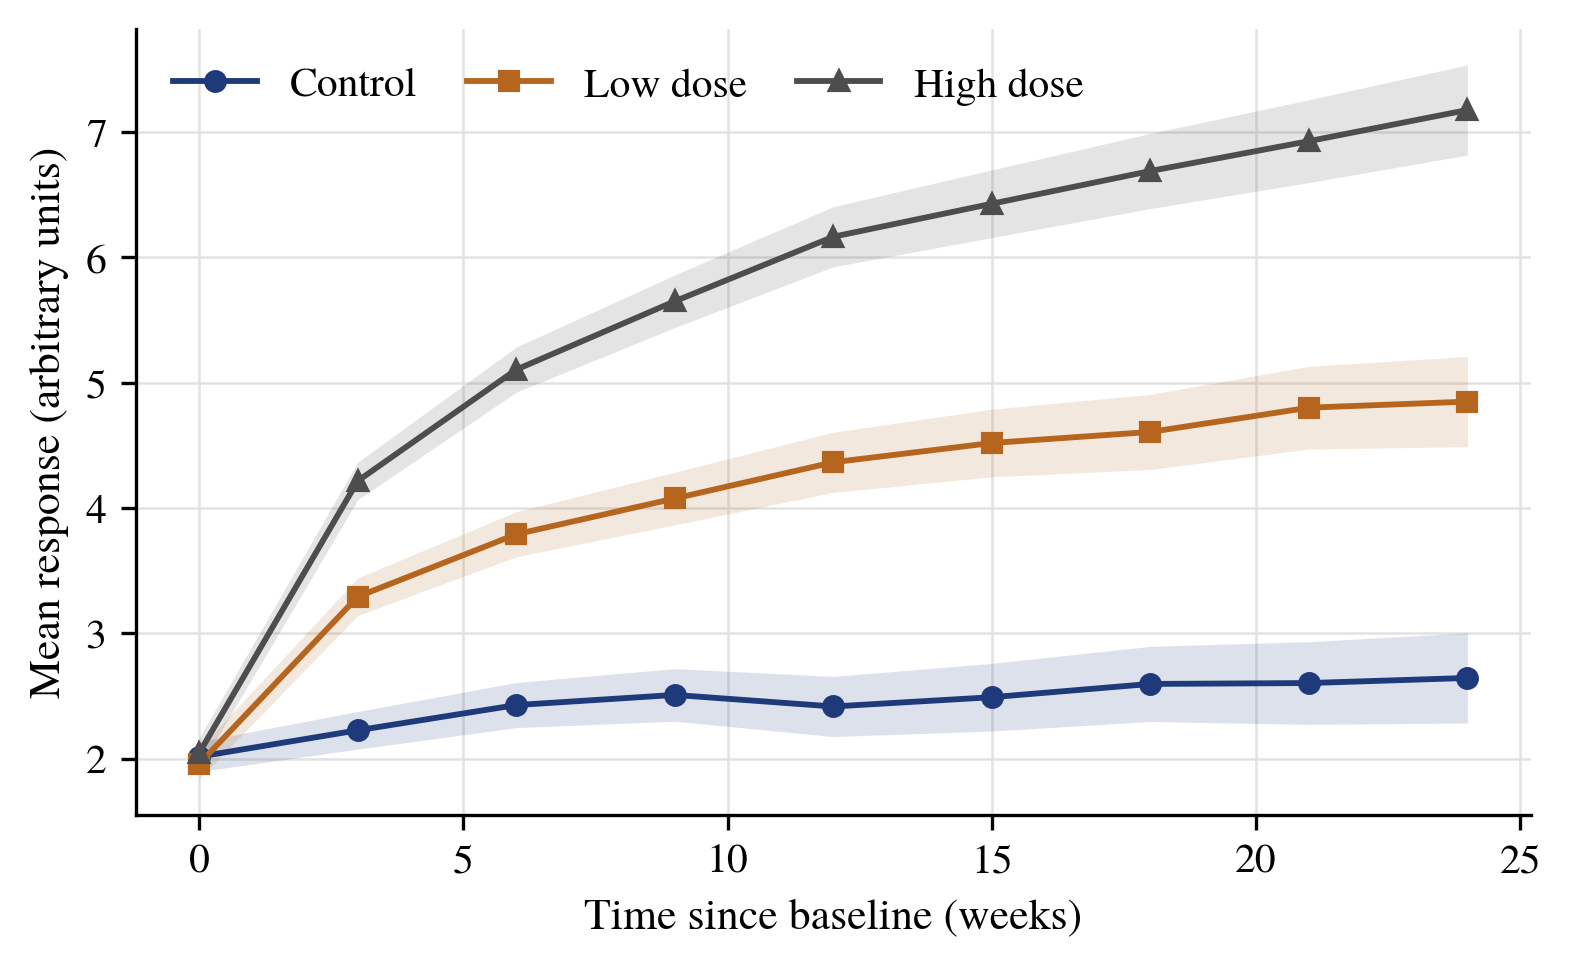
\includegraphics[width=0.85\linewidth]{figures/fig1-timecourse.png}
  \caption{Mean response over time by condition; shaded bands show $\pm$1 SE.
  Synthetic example data: replace with your own figure.}\label{fig:timecourse}
\end{figure}

\begin{figure}[htbp]
  \centering
  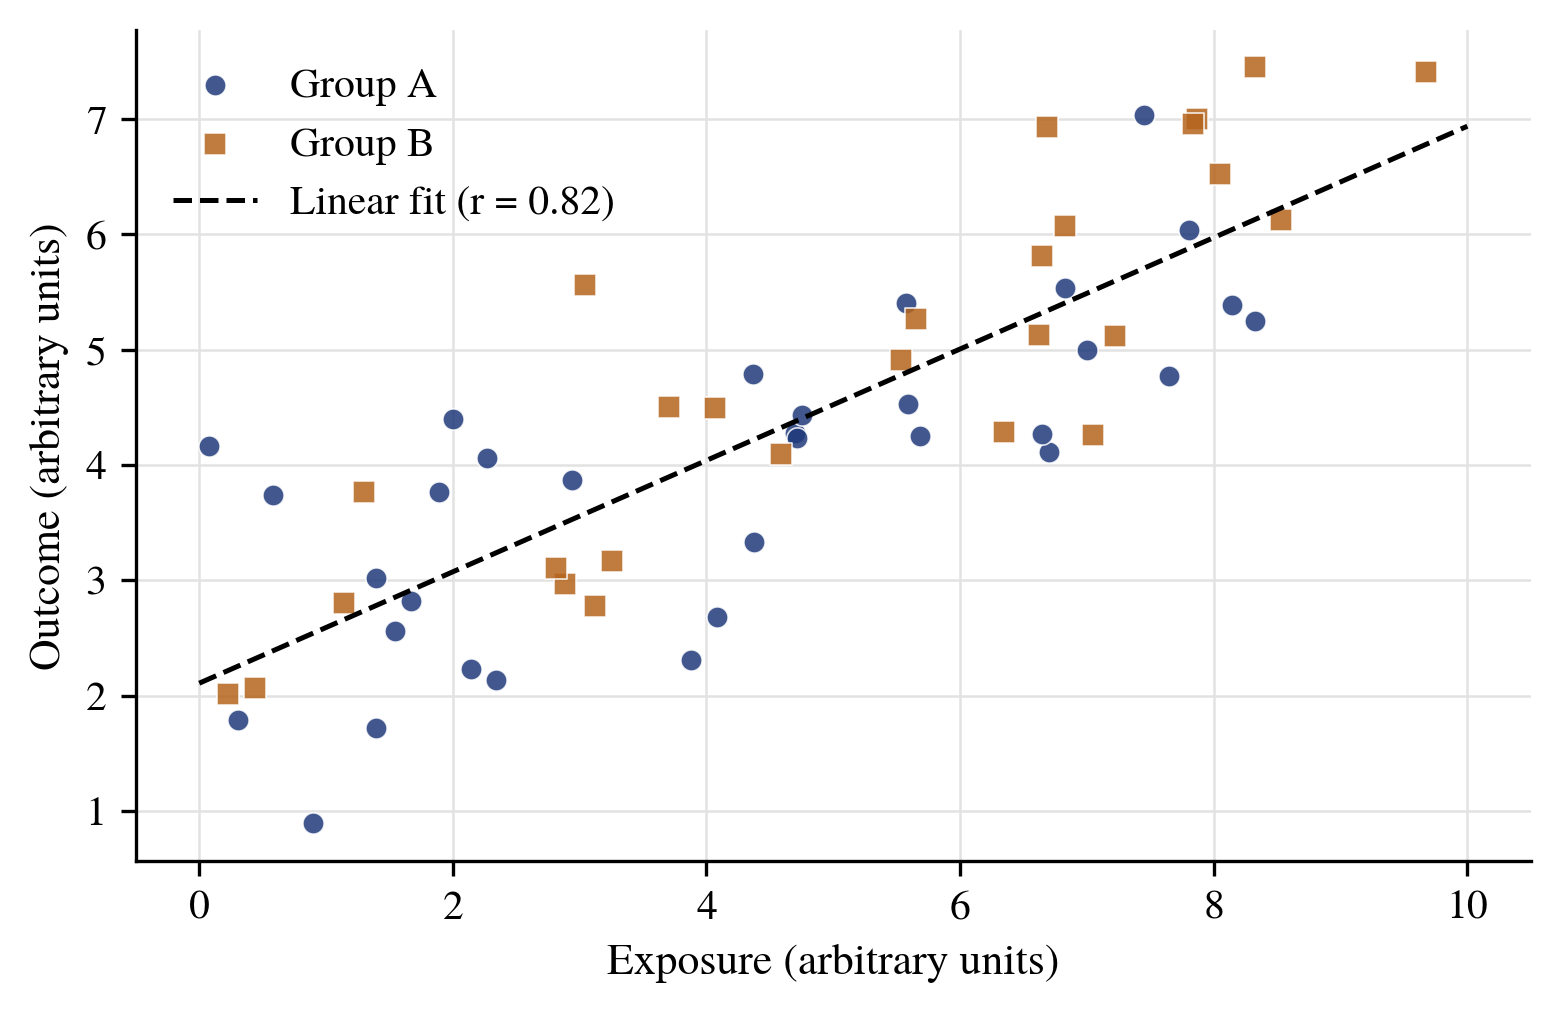
\includegraphics[width=0.85\linewidth]{figures/fig2-scatter.png}
  \caption{Outcome versus exposure for two groups, with a linear fit (dashed).
  Synthetic example data: replace with your own figure.}\label{fig:scatter}
\end{figure}

\subsection{Group comparison}
Figure~\ref{fig:comparison} compares the groups; the effect size follows
Equation~\eqref{eq:effect}.

\begin{figure}[htbp]
  \centering
  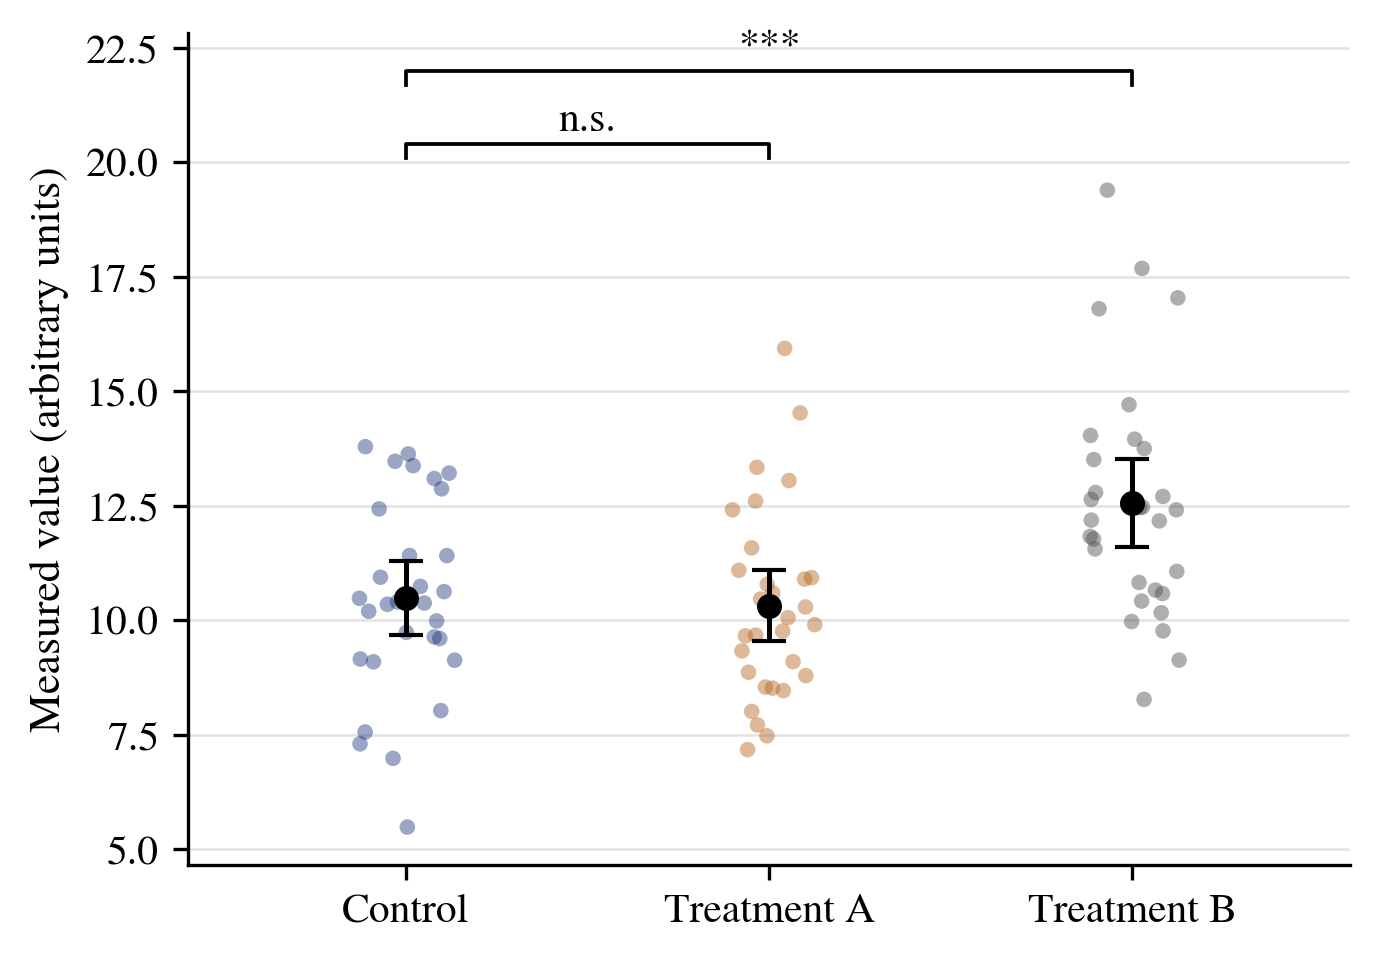
\includegraphics[width=0.65\linewidth]{figures/fig3-comparison.png}
  \caption{Group means with 95\% confidence intervals (black) and individual
  observations (coloured). Brackets show permutation-test results
  (n.s., not significant; $^{*}p<0.05$; $^{**}p<0.01$; $^{***}p<0.001$).
  Synthetic example data: replace with your own figure.}\label{fig:comparison}
\end{figure}

\section{Discussion}\label{sec:discussion}
Interpret the findings in light of the literature~\cite{author2020,book2018}.
Discuss limitations, generalisability and implications for future work.

\section{Conclusions}
State the main conclusions concisely, without repeating the abstract.

\section*{Acknowledgments}
Thank colleagues, technicians and facilities that do not meet authorship criteria.

\section*{Funding}
This work was supported by [funder name] under grant number [000000].
The funder had no role in the study design, analysis or decision to publish.

\section*{Conflict of interest}
The authors declare that they have no competing interests.
(Or: describe any financial or personal relationships that could be perceived as a conflict.)

\section*{Data availability}
The data supporting this study are available at [repository, DOI or URL]. Analysis
code is available at [repository URL].

\section*{Supplementary material}
Supplementary Table~S1 lists the full participant characteristics, and
Supplementary Figure~S1 shows additional diagnostic plots. Both are provided as
separate files with the submission.

\singlespacing
\bibliographystyle{unsrtnat}
\bibliography{research-manuscript}
\doublespacing

% ---- Optional appendices: delete if not needed ----
\appendix
\renewcommand{\theequation}{A\arabic{equation}}
\setcounter{equation}{0}

\section{Additional methodological details}\label{app:details}
Provide derivations or protocols that would interrupt the main text. For
example, a model with a covariate $x_{ij}$ extends Equation~\eqref{eq:model}:
\begin{equation}\label{eq:ancova}
  y_{ij} = \mu + \tau_i + \beta\,(x_{ij}-\bar{x}) + \varepsilon_{ij}.
\end{equation}

\end{document}
